% --------------------------------------------------------------
% This is all preamble stuff that you don't have to worry about.
% Head down to where it says "Start here"
% --------------------------------------------------------------
 
\documentclass[12pt]{article}
 
\usepackage[margin=1in]{geometry} 
\usepackage{amsmath,amsthm,amssymb}
\usepackage[utf8]{inputenc}
\usepackage[spanish]{babel}
\usepackage{graphicx}
%\usepackage[dvipsnames]{xcolor}
%\usepackage[american,siunitx]{circuitikz}
 
\newcommand{\N}{\mathbb{N}}
\newcommand{\Z}{\mathbb{Z}}
 
\newenvironment{theorem}[2][Theorem]{\begin{trivlist}
\item[\hskip \labelsep {\bfseries #1}\hskip \labelsep {\bfseries #2.}]}{\end{trivlist}}
\newenvironment{lemma}[2][Lemma]{\begin{trivlist}
\item[\hskip \labelsep {\bfseries #1}\hskip \labelsep {\bfseries #2.}]}{\end{trivlist}}
\newenvironment{exercise}[2][Exercise]{\begin{trivlist}
\item[\hskip \labelsep {\bfseries #1}\hskip \labelsep {\bfseries #2.}]}{\end{trivlist}}
\newenvironment{reflection}[2][Reflection]{\begin{trivlist}
\item[\hskip \labelsep {\bfseries #1}\hskip \labelsep {\bfseries #2.}]}{\end{trivlist}}
\newenvironment{proposition}[2][Proposition]{\begin{trivlist}
\item[\hskip \labelsep {\bfseries #1}\hskip \labelsep {\bfseries #2.}]}{\end{trivlist}}
\newenvironment{corollary}[2][Corollary]{\begin{trivlist}
\item[\hskip \labelsep {\bfseries #1}\hskip \labelsep {\bfseries #2.}]}{\end{trivlist}}
 
\begin{document}
 
% --------------------------------------------------------------
%                         Start here
% --------------------------------------------------------------
 
%\renewcommand{\qedsymbol}{\filledbox}
 
\title{Tarea 2}%replace X with the appropriate number
\author{Víctor de Jesús Medrano Zarazúa\\ %replace with your name
Análisis y diseño de circuitos - Definición de nodos, ramas, lazos y mallas} %if necessary, replace with your course title
 
\maketitle

\begin{itemize}
    \item \textbf{Investigar los conceptos de: } Nodo, rama, lazo, malla, circuito abierto, circuito cerrado y corto circuito.

    \item Determinar número de nodos, ramas, lazos y mallas en cada circuito.

    \begin{figure}[h!]
        \centering
        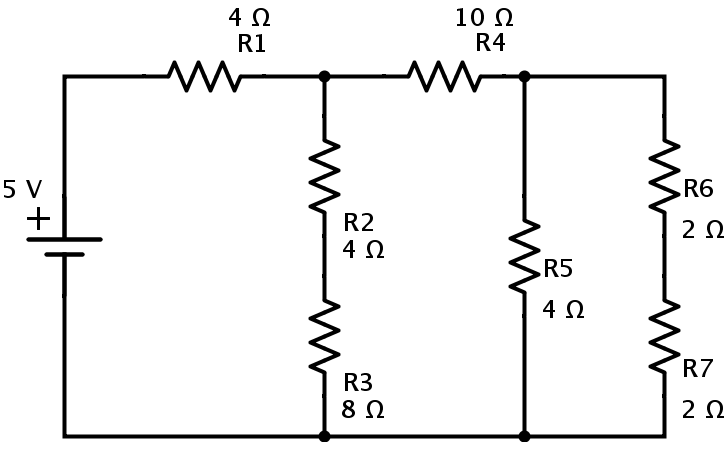
\includegraphics [scale=0.45]{circuit_1}
        %\caption{Sección de Issues}
        \label{fig:circuit1}
    \end{figure}

    \begin{figure}[h!]
        \centering
        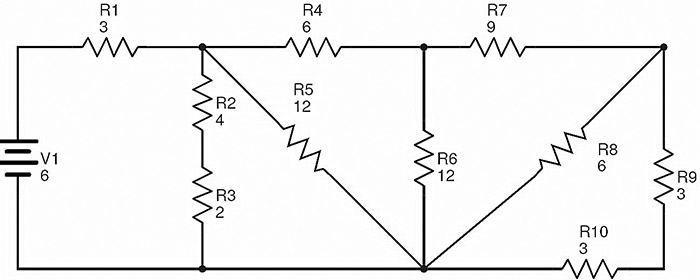
\includegraphics [scale=0.55]{circuit_2}
        %\caption{Sección de Issues}
        \label{fig:circuit2}
    \end{figure}
    \newpage
    \vspace{-2in}
    \begin{figure}[h!]
        \centering
        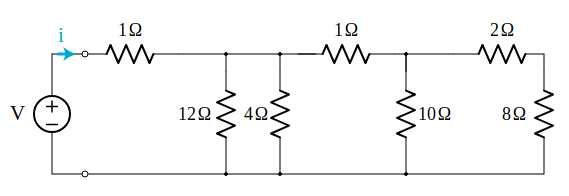
\includegraphics [scale=0.75]{circuit_3}
        %\caption{Sección de Issues}
        \label{fig:circuit3}
    \end{figure}

\end{itemize}

% --------------------------------------------------------------
%     You don't have to mess with anything below this line.
% --------------------------------------------------------------
 
\end{document}
